\documentclass[11pt,a4paper]{article}

\usepackage[utf8]{inputenc}
\usepackage[T1]{fontenc}
\usepackage{lmodern}
\usepackage[french]{babel}
\usepackage[margin=2.3cm]{geometry}
\usepackage{microtype}
\usepackage{amsmath}
\usepackage{graphicx}
\usepackage{booktabs}
\usepackage{float}
\usepackage[font=small,labelfont=bf]{caption}
\usepackage{enumitem}
\usepackage{xcolor}
\usepackage{listings}
\usepackage[hidelinks]{hyperref}

\graphicspath{{figures/}}
\setlist{itemsep=2pt,topsep=4pt}
\lstset{basicstyle=\ttfamily\small,columns=fullflexible,frame=single,framerule=0.4pt,backgroundcolor=\color{gray!6}}
\newcommand{\logg}{$\log g$}
\newcommand{\teff}{$T_{\mathrm{eff}}$}
\newcommand{\mh}{[M/H]}

\title{\textbf{Classification d'étoiles à partir des spectres APOGEE DR17}\\[4pt]
\large Version complète : catalogue allStar et 100\,000 étoiles}
\author{Félix Dubé \and Imran Akki \and Charles-Antoine Fournier \and Youssef Lahrichi \and Bastien Posez}
\date{Projet de session, GIF-4101 / GIF-7005 / GIF-7015\\Université Laval, décembre 2026}

\begin{document}
\maketitle

\begin{abstract}
\noindent Nous classons des étoiles à partir de leur seul spectre infrarouge APOGEE DR17, avec et sans étiquettes, sur 99\,773 spectres. Le catalogue complet \texttt{allStar} fournit trois informations absentes de la version allégée : l'ajustement brut FPARAM, qui étiquette les mauvais spectres, les abondances [Mg/Fe] et [Fe/H], et les distances Gaia. Sans étiquettes, un mélange gaussien sur 10 composantes PCA retrouve les classes évolutives avec un ARI de 0,44 à quatre groupes. Avec étiquettes, un CNN 1-D atteint un macro F1 de 0,86 quand il s'entraîne sur tous les spectres, contre 0,78 pour une forêt aléatoire. Tripler l'échantillon fait passer le macro F1 du CNN de 0,82 à 0,83 et celui de la forêt de 0,70 à 0,75. L'effet des mauvais spectres dépend de la tâche : ils aident la classification à tous les SNR, mais dégradent la régression sur les bons spectres (erreur sur \teff{} de 33 à 54\,K), car leurs étiquettes sont bruitées.
\end{abstract}

\tableofcontents
\newpage

%=====================================================================
\section{Introduction}

APOGEE DR17 publie les spectres infrarouges de 657\,000 étoiles \cite{dr17,majewski2017}. Le pipeline ASPCAP \cite{aspcap} en tire la température effective \teff{}, la gravité de surface \logg{} et la métallicité \mh{}, en ajustant des modèles d'atmosphère. Notre question : un algorithme regroupe-t-il les étoiles en classes physiques à partir du spectre seul ?

Garcia-Dias et al.\ \cite{garciadias2018} ont montré que K-means sépare naines, sous-géantes, red clump et branche des géantes rouges dans APOGEE. Ils signalaient deux limites : le résultat dépend de l'initialisation, et le nombre de groupes reste difficile à choisir.

Une première version de notre projet utilisait le catalogue allégé \texttt{allStarLite} et 30\,781 étoiles. Cette version complète apporte trois changements :
\begin{enumerate}
  \item Le catalogue complet \texttt{allStar} (4\,Go) remplace \texttt{allStarLite} (1,8\,Go).
  \item L'échantillon passe à 99\,773 étoiles.
  \item Les étiquettes s'enrichissent : FPARAM pour les mauvais spectres, [Mg/Fe] et [Fe/H] pour les disques, distances Gaia pour le bulbe.
\end{enumerate}

Le protocole reste le même : réduction de dimension, clustering validé a posteriori, apprentissage supervisé, et étude de l'impact de la qualité des spectres.

%=====================================================================
\section{Données}

\subsection{APOGEE DR17 et le catalogue complet}

APOGEE observe en bande H (15\,150 à 16\,940\,Å) à une résolution $R \approx 22\,500$, depuis Apache Point (nord) et Las Campanas (sud). Chaque spectre normalisé (\texttt{aspcapStar}) compte 8\,575 pixels sur une grille log-linéaire :
\begin{equation}
  \log_{10} \lambda_i = 4{,}179 + 6 \times 10^{-6}\, i, \qquad i = 0, \dots, 8\,574.
\end{equation}

Le catalogue complet \texttt{allStar} compte 733\,901 lignes et 234 colonnes. Nous en utilisons quatre de plus que la version allégée :

\begin{table}[H]
\centering
\begin{tabular}{ll}
\toprule
Colonne & Usage \\
\midrule
\texttt{FPARAM} & ajustement brut d'ASPCAP, publié même pour les étoiles \texttt{STAR\_BAD} \\
\texttt{FE\_H}, \texttt{MG\_FE} & abondances, pour séparer disque mince et disque épais \\
\texttt{GAIAEDR3\_R\_MED\_GEO} & distance Gaia EDR3, pour placer le bulbe \\
\bottomrule
\end{tabular}
\caption{Colonnes du catalogue complet ajoutées à cette version.}
\end{table}

Nous avons vérifié l'ordre de \texttt{FPARAM} par corrélation avec les valeurs publiées sur 20\,000 étoiles : l'indice 0 donne \teff{} (corrélation 0,999), l'indice 1 \logg{} (0,991) et l'indice 3 \mh{} (1,000). FPARAM n'est pas calibré : son \teff{} est en médiane 75\,K plus bas que le \teff{} publié, et son \logg{} 0,04\,dex plus haut.

\subsection{Échantillon et qualité}

Nous excluons le télescope de 1\,m, les doublons, les standards telluriques et les spectres de SNR inférieur à 5. Nous tirons au hasard (graine 42) 66\,000 bons et 33\,000 mauvais spectres, et nous ajoutons les 785 membres d'amas ouverts OCCAM \cite{occam}. Le serveur SDSS fournit 99\,773 des 99\,785 spectres demandés.

Un bon spectre vérifie quatre critères : SNR $\geq 70$, \texttt{STARFLAG} $= 0$, pas de \texttt{STAR\_BAD} dans \texttt{ASPCAPFLAG}, \teff{} et \logg{} publiés. L'échantillon compte 66\,372 bons et 33\,401 mauvais spectres. 69\,\% des mauvais spectres ont un SNR $\geq 70$ : un drapeau les écarte, pas le bruit. Le SNR médian vaut 168 pour les bons et 103 pour les mauvais, et la fraction moyenne de pixels douteux 3,1\,\% et 5,6\,\%.

\subsection{Étiquettes}

\paragraph{Origine.} ASPCAP ne publie pas \teff{} ni \logg{} pour les étoiles \texttt{STAR\_BAD}. Nous complétons ces valeurs avec FPARAM. La qualité se décide avant ce complément. Au total, 96\,958 étoiles portent une étiquette ASPCAP et 2\,815 une étiquette FPARAM. Seules 12 étoiles restent sans classe, contre 802 dans la première version.

\paragraph{Classes évolutives.} Naine si $\log g \geq 4{,}0$, sous-géante si $3{,}5 \leq \log g < 4{,}0$, red clump si $\log g < 3{,}5$ et présente dans le catalogue red clump DR17 \cite{bovy2014}, géante rouge (RGB) sinon. Les bons spectres comptent 19\,804 naines, 3\,590 sous-géantes, 36\,808 RGB et 6\,170 étoiles du red clump.

\paragraph{Populations.} Nous séparons disque mince et disque épais par la ligne de Weinberg et al.\ \cite{weinberg2019} : disque épais si $[\text{Mg/Fe}] > 0{,}12 - 0{,}13\,\min([\text{Fe/H}], 0)$. Le halo regroupe les étoiles de $[\text{Fe/H}] < -1$. Le bulbe regroupe les étoiles de $[\text{Fe/H}] \geq -1$ situées à moins de 3\,kpc du centre galactique, avec
\begin{equation}
  R_{\mathrm{GC}} = \sqrt{(R_0 - d\cos b \cos l)^2 + (d \cos b \sin l)^2 + (d \sin b)^2}, \qquad R_0 = 8{,}2\ \text{kpc},
\end{equation}
où $d$ est la distance Gaia EDR3. Les bons spectres comptent 47\,258 étoiles du disque mince, 13\,385 du disque épais, 2\,682 du bulbe et 2\,144 du halo.

\paragraph{Amas ouverts.} Un membre OCCAM a une probabilité supérieure à 0,5 en vitesse radiale, en [Fe/H] et en mouvement propre.

\subsection{Prétraitement et découpage}

Nous retirons les 1\,061 pixels des trous entre détecteurs (il reste 7\,514 pixels), remplaçons chaque pixel douteux par 1, le niveau du continuum, et bornons le flux entre 0 et 1,5. Les réseaux reçoivent $1 - F_\lambda$. Un découpage unique 70 / 15 / 15 sépare entraînement, validation et test. La validation contient les bons spectres seulement. Le test compte 9\,997 bons spectres classés (\texttt{test\_good}) et 14\,968 spectres en tout (\texttt{test\_all}).

%=====================================================================
\section{Méthodes}

Les méthodes reprennent celles de la première version.

\begin{itemize}
  \item \textbf{Réduction de dimension.} PCA à 50 composantes (75,2\,\% de variance avec 10), puis t-SNE \cite{tsne} sur 10\,000 étoiles.
  \item \textbf{Autoencodeur.} Réseau dense $7\,514 \to 512 \to 128 \to 16$ et retour, perte quadratique, 30 époques.
  \item \textbf{Clustering.} K-means, mélange gaussien à covariances pleines (GMM) et HDBSCAN \cite{hdbscan}, sur 10 composantes PCA standardisées ou sur le latent de l'autoencodeur. Choix de $k$ par silhouette, stabilité mesurée par l'ARI moyen entre 10 graines de K-means.
  \item \textbf{Validation.} ARI \cite{ari}, NMI, et pureté des amas ouverts.
  \item \textbf{Supervisé.} Forêt aléatoire de 300 arbres sur 50 composantes PCA, et CNN 1-D de 150\,000 paramètres (3 blocs convolutifs, 30 époques, Adam). Deux tâches : 4 classes, et régression de \teff{}, \logg{}, \mh{}.
  \item \textbf{Qualité.} Chaque modèle s'entraîne sur les bons spectres (46\,331 étoiles classées), puis sur tous (69\,842).
\end{itemize}

%=====================================================================
\section{Résultats}

\subsection{Exploration}

\begin{figure}[H]
\centering
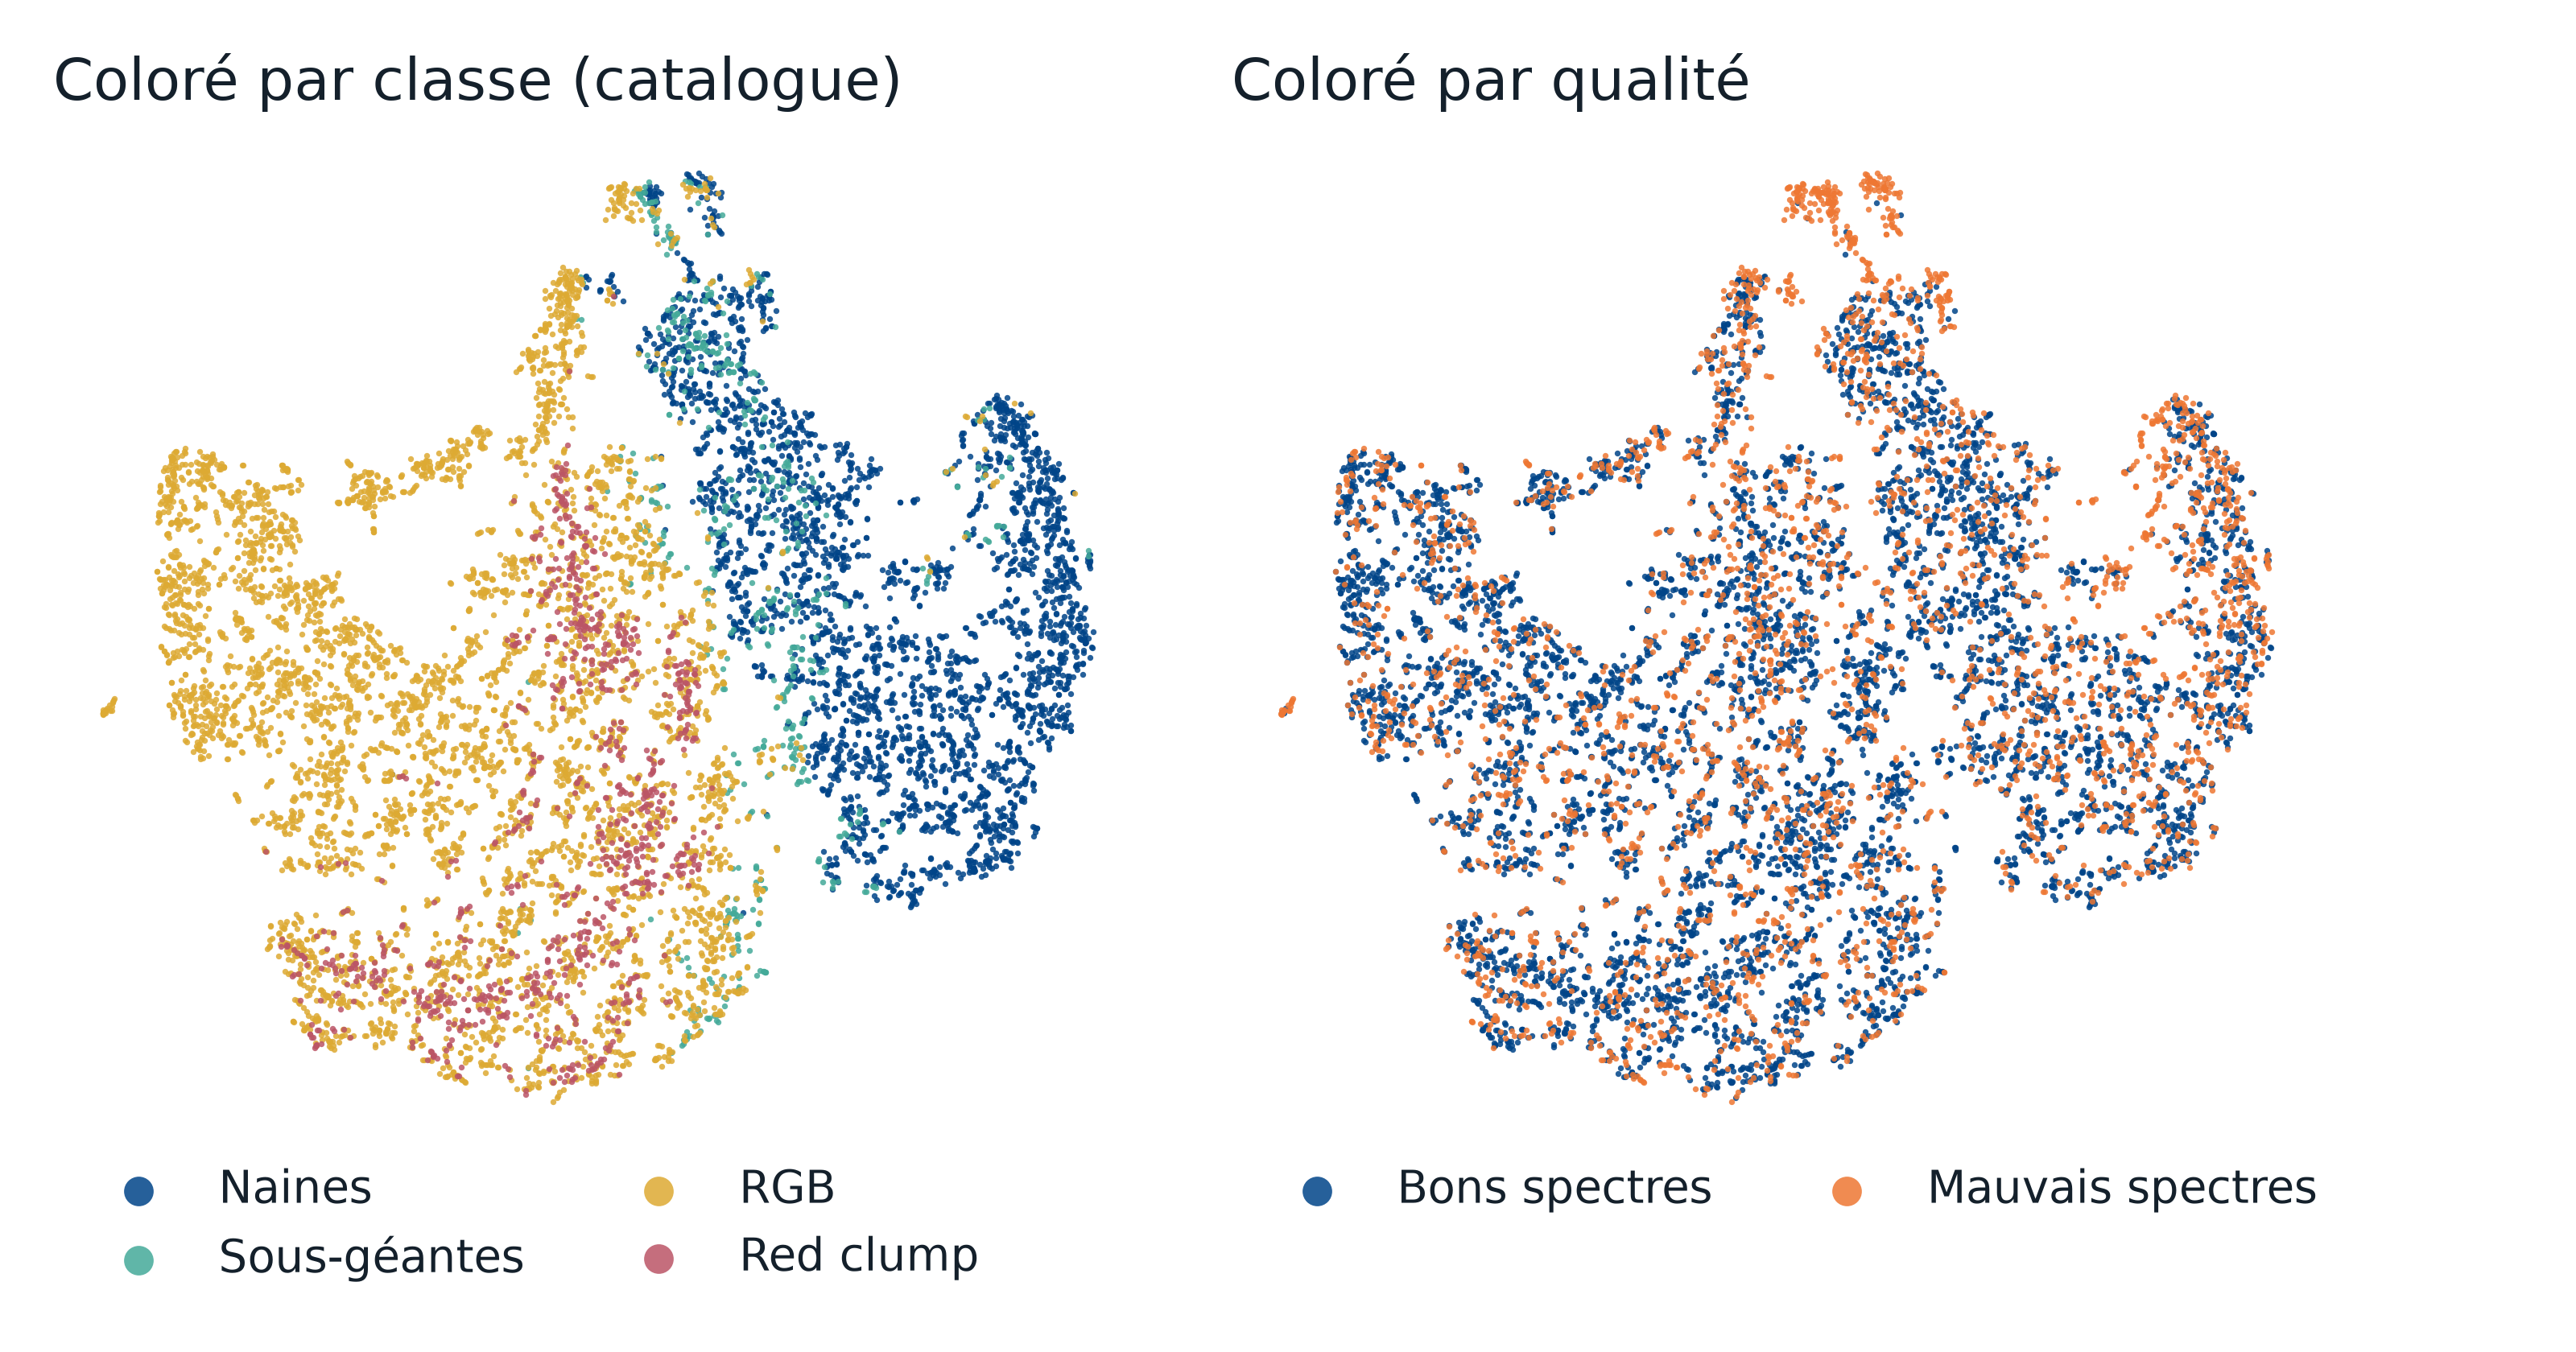
\includegraphics[width=\linewidth]{tsne.png}
\caption{t-SNE de 10\,000 étoiles. Gauche : classes du catalogue. Droite : qualité.}
\label{fig:tsne}
\end{figure}

Le t-SNE (figure~\ref{fig:tsne}) sépare naines et géantes sans étiquette. Les sous-géantes forment la frontière. Le red clump reste mêlé à la RGB. Les mauvais spectres se mêlent aux bons, avec quelques îlots en bordure.

\subsection{Clustering}

\begin{table}[H]
\centering
\begin{tabular}{llrrr}
\toprule
Entrée & Méthode & ARI & NMI & Pureté OCCAM \\
\midrule
PCA, bons, $k = 4$ & GMM & \textbf{0,44} & \textbf{0,56} & 0,93 \\
PCA, bons, $k = 3$ & GMM & 0,42 & 0,53 & 0,90 \\
PCA, bons, $k = 3$ & K-means & 0,08 & 0,26 & 0,95 \\
PCA, bons, $k = 4$ & K-means & 0,06 & 0,25 & 0,89 \\
PCA, bons & HDBSCAN (25\,\% de bruit) & $-0{,}04$ & 0,03 & 0,73 \\
Latent, bons, $k = 2$ & K-means & $-0{,}07$ & 0,12 & 1,00 \\
PCA, tous, $k = 4$ & GMM & 0,14 & 0,27 & 0,88 \\
PCA, tous, $k = 4$ & K-means & 0,03 & 0,22 & 0,96 \\
\bottomrule
\end{tabular}
\caption{Validation du clustering contre les classes évolutives.}
\label{tab:cluster}
\end{table}

Le GMM sur PCA reste la meilleure méthode (tableau~\ref{tab:cluster}). À $k = 4$, le nombre de classes réelles, il atteint un ARI de 0,44. À $k = 3$, ses groupes suivent la séquence principale, le haut de la RGB, et le red clump avec le bas de la RGB (tableau~\ref{tab:gmm}, figure~\ref{fig:kiel}).

\begin{table}[H]
\centering
\begin{tabular}{lrrrr}
\toprule
Groupe & Naines & Sous-géantes & RGB & Red clump \\
\midrule
A : séquence principale & 19\,800 & 2\,934 & 1\,833 & 48 \\
B : haut de la RGB & 1 & 5 & 14\,831 & 123 \\
C : red clump et bas de la RGB & 3 & 651 & 20\,144 & 5\,999 \\
\bottomrule
\end{tabular}
\caption{Composition des groupes du GMM à $k = 3$ (PCA, bons spectres).}
\label{tab:gmm}
\end{table}

\begin{figure}[H]
\centering
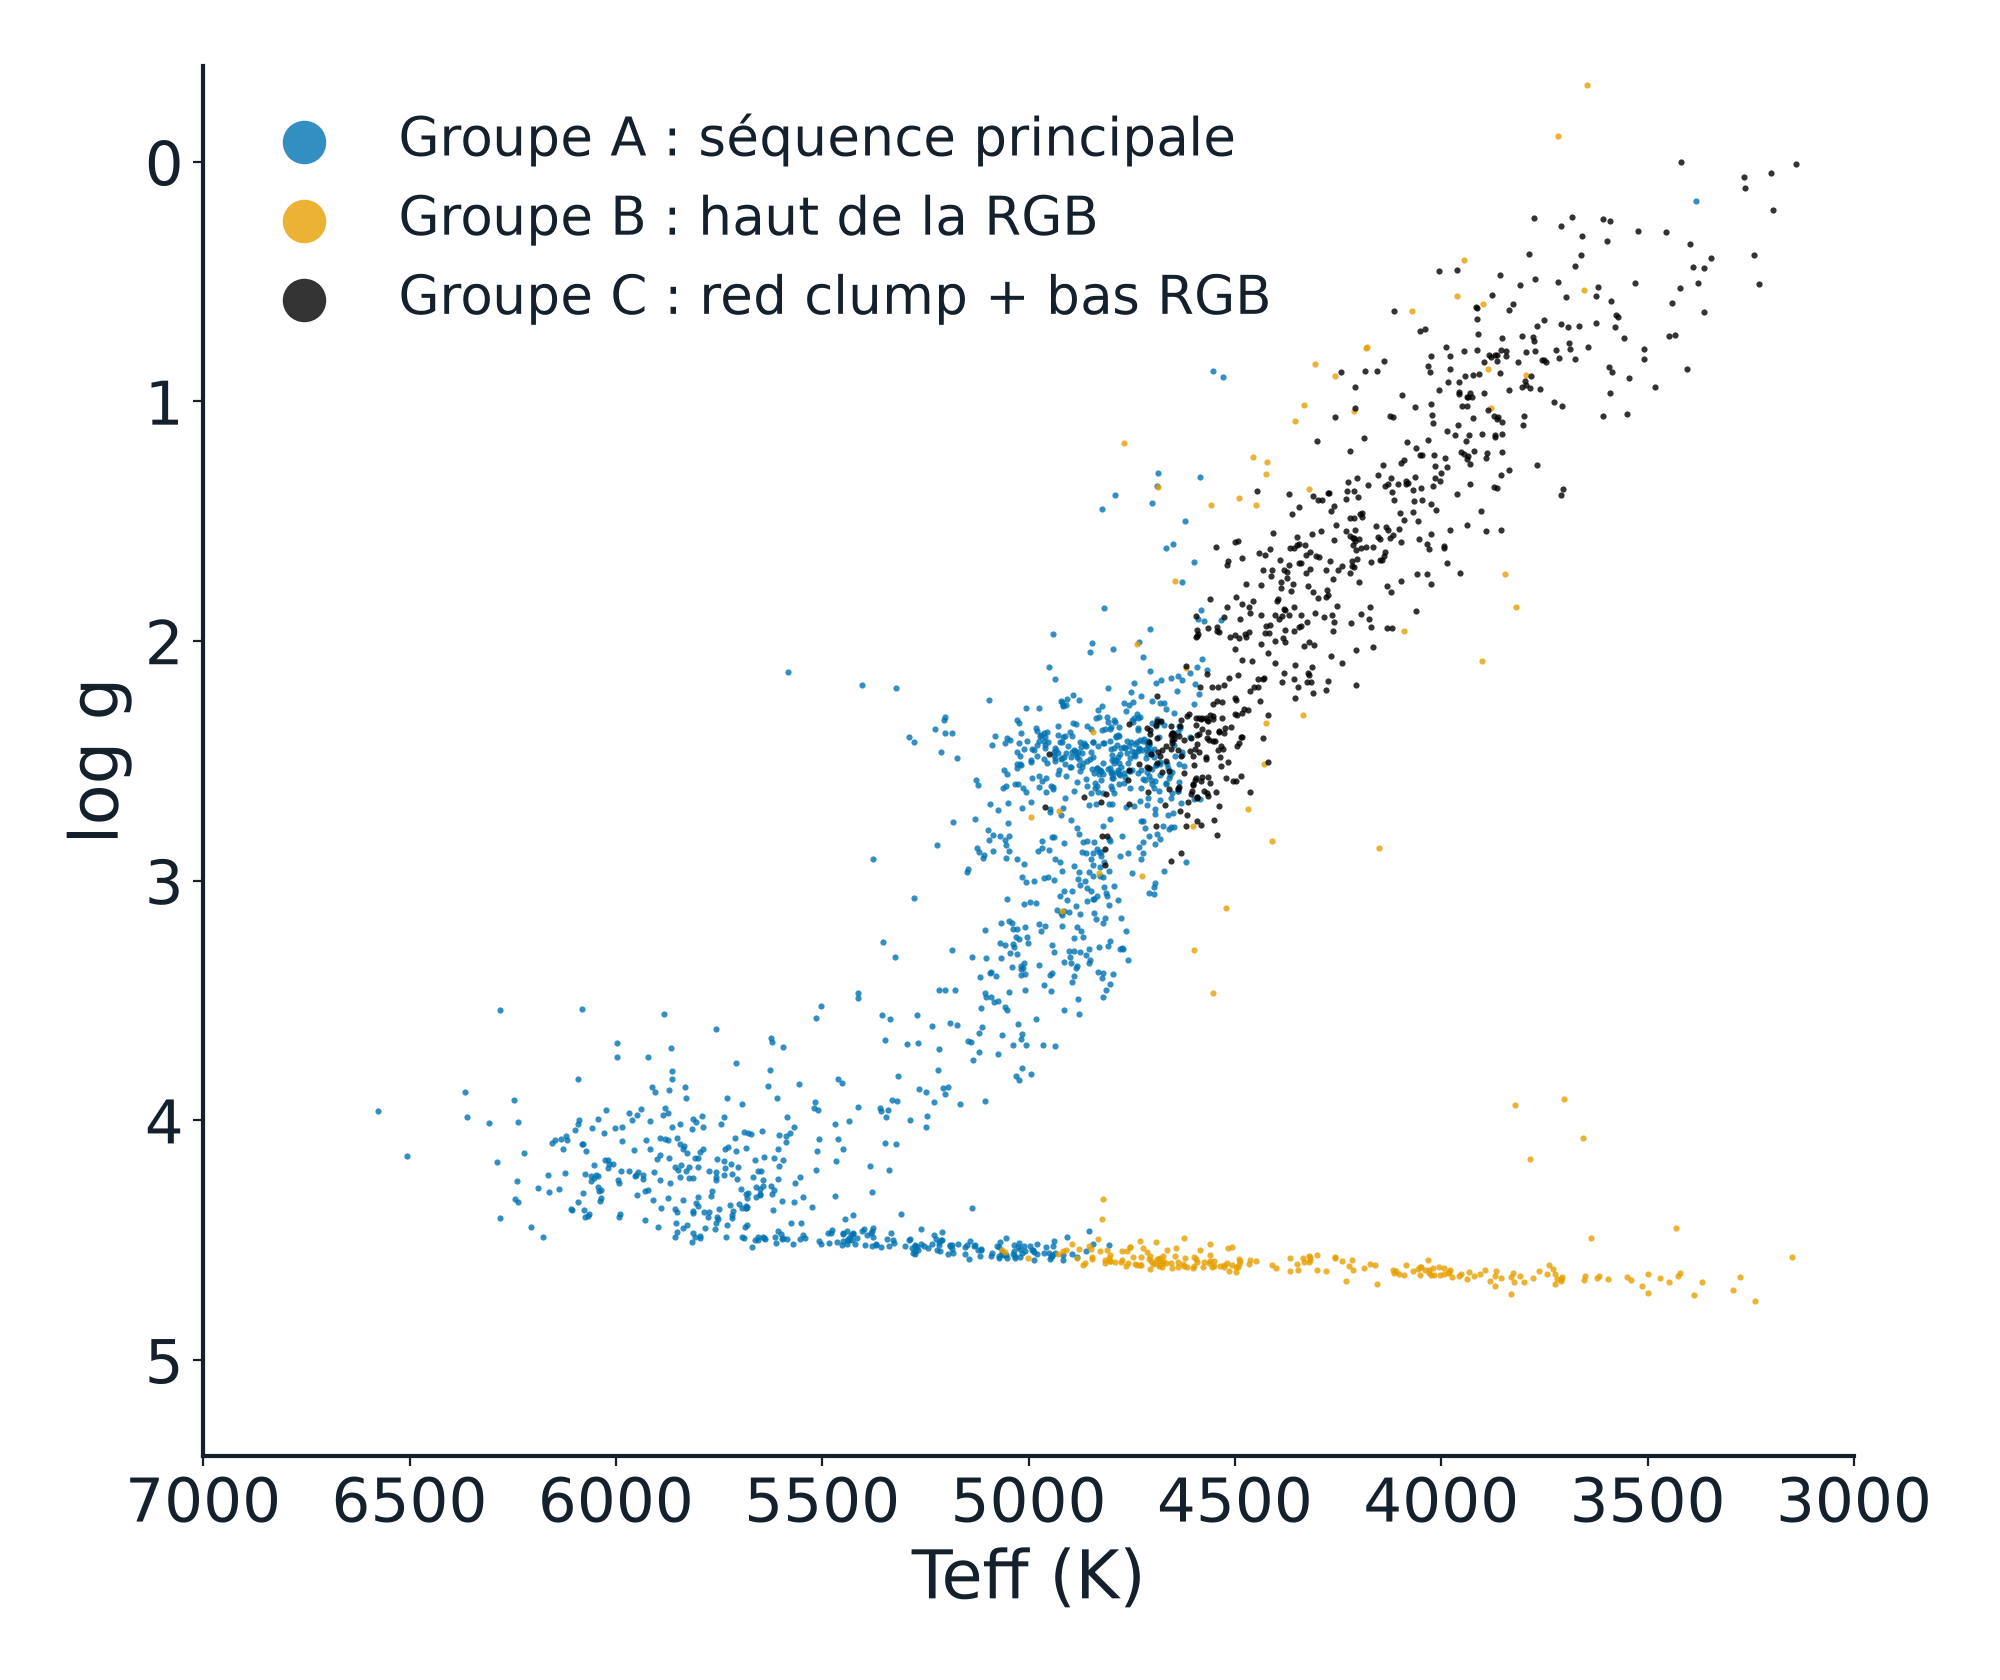
\includegraphics[width=0.6\linewidth]{kiel_gmm.png}
\caption{Diagramme de Kiel des bons spectres, coloré par les groupes du GMM à $k = 3$.}
\label{fig:kiel}
\end{figure}

La silhouette reste basse (maximum 0,28 à $k = 3$) : les spectres forment un continuum. La stabilité de K-means vaut 0,30 à $k = 2$, 0,47 à $k = 3$ et 0,80 à $k = 4$ (figure~\ref{fig:scan}). Comme dans la première version, $k = 4$ est le choix le plus stable.

\begin{figure}[H]
\centering
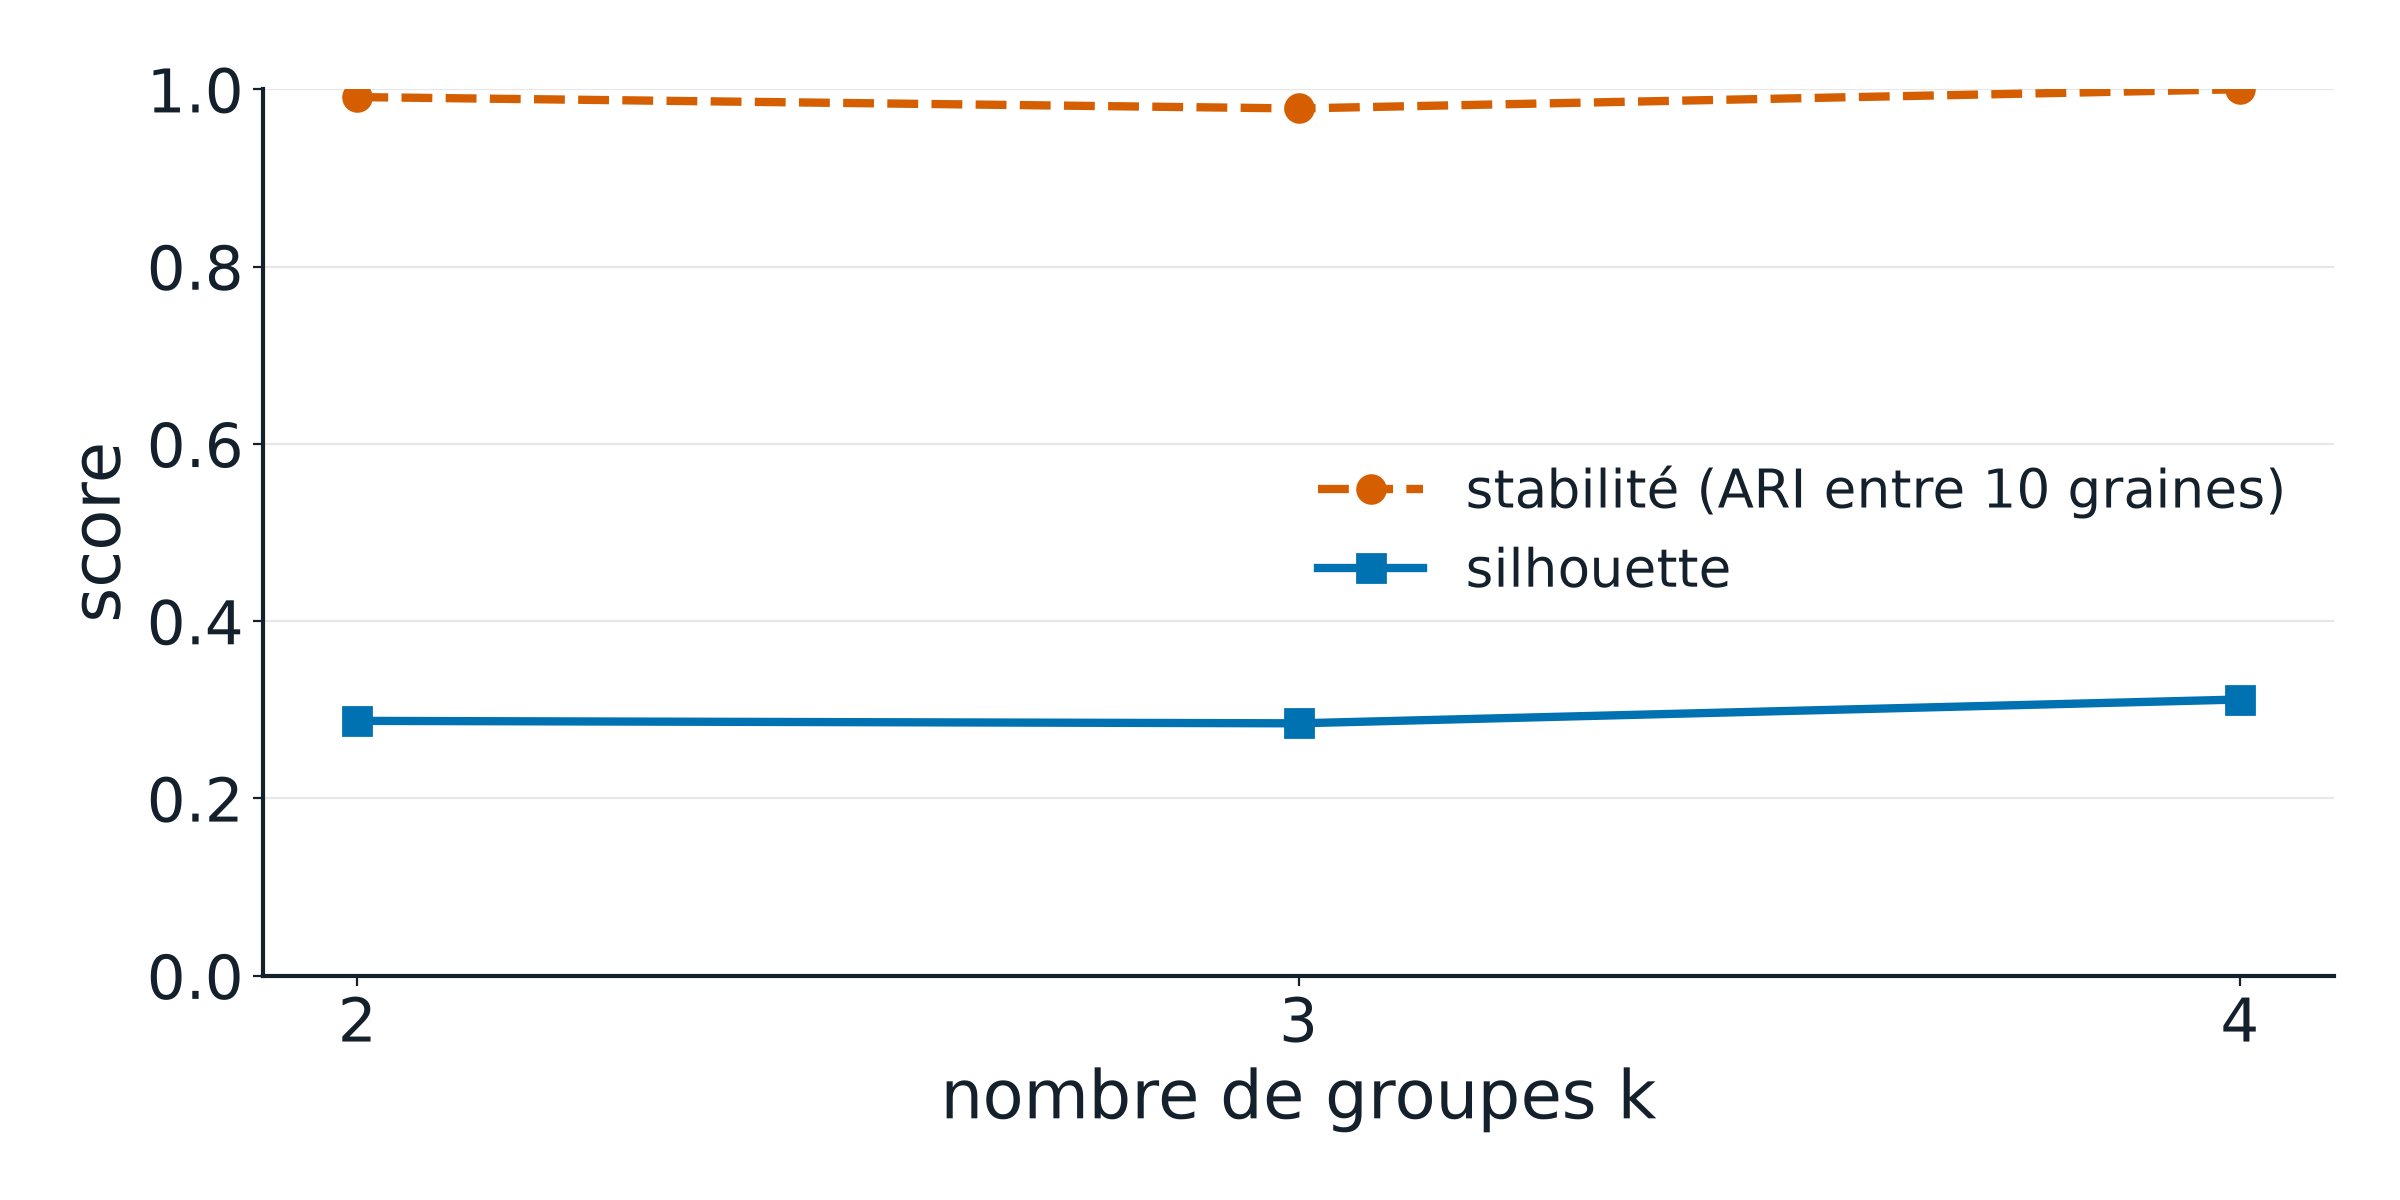
\includegraphics[width=0.72\linewidth]{kmeans_scan.png}
\caption{Silhouette et stabilité de K-means selon $k$ (PCA, bons spectres).}
\label{fig:scan}
\end{figure}

Les nouvelles étiquettes de population ne changent pas le constat : aucune méthode ne les retrouve (ARI $\leq 0{,}13$). [Mg/Fe] diffère d'environ 0,1 à 0,2\,dex entre les disques, un effet faible face aux variations de \teff{} et de \logg{}.

Sur tous les spectres, la silhouette choisit $k = 4$. K-means forme alors un groupe de 12\,699 géantes et un groupe de 273 géantes isolées, et l'ARI tombe à 0,03.

\subsection{Apprentissage supervisé}

\begin{table}[H]
\centering
\begin{tabular}{llrrrrr}
\toprule
Modèle & Entraînement & Accuracy & Macro F1 & \teff{} (K) & \logg{} (dex) & \mh{} (dex) \\
\midrule
Forêt & bons & 0,892 & 0,751 & 30,0 & 0,131 & 0,047 \\
Forêt & tous & 0,899 & 0,778 & \textbf{28,1} & 0,108 & 0,042 \\
CNN 1-D & bons & 0,907 & 0,834 & 32,9 & \textbf{0,069} & \textbf{0,025} \\
CNN 1-D & tous & \textbf{0,911} & \textbf{0,860} & 53,7 & 0,102 & 0,030 \\
\bottomrule
\end{tabular}
\caption{Résultats sur \texttt{test\_good} (9\,997 étoiles). Erreurs absolues moyennes par rapport à ASPCAP.}
\label{tab:sup}
\end{table}

Le CNN bat la forêt en classification et sur \logg{} et \mh{} (tableau~\ref{tab:sup}). La forêt garde l'avantage sur \teff{}. Notre hypothèse : \teff{} domine la variance du spectre, et les premières composantes PCA la portent déjà.

\begin{figure}[H]
\centering
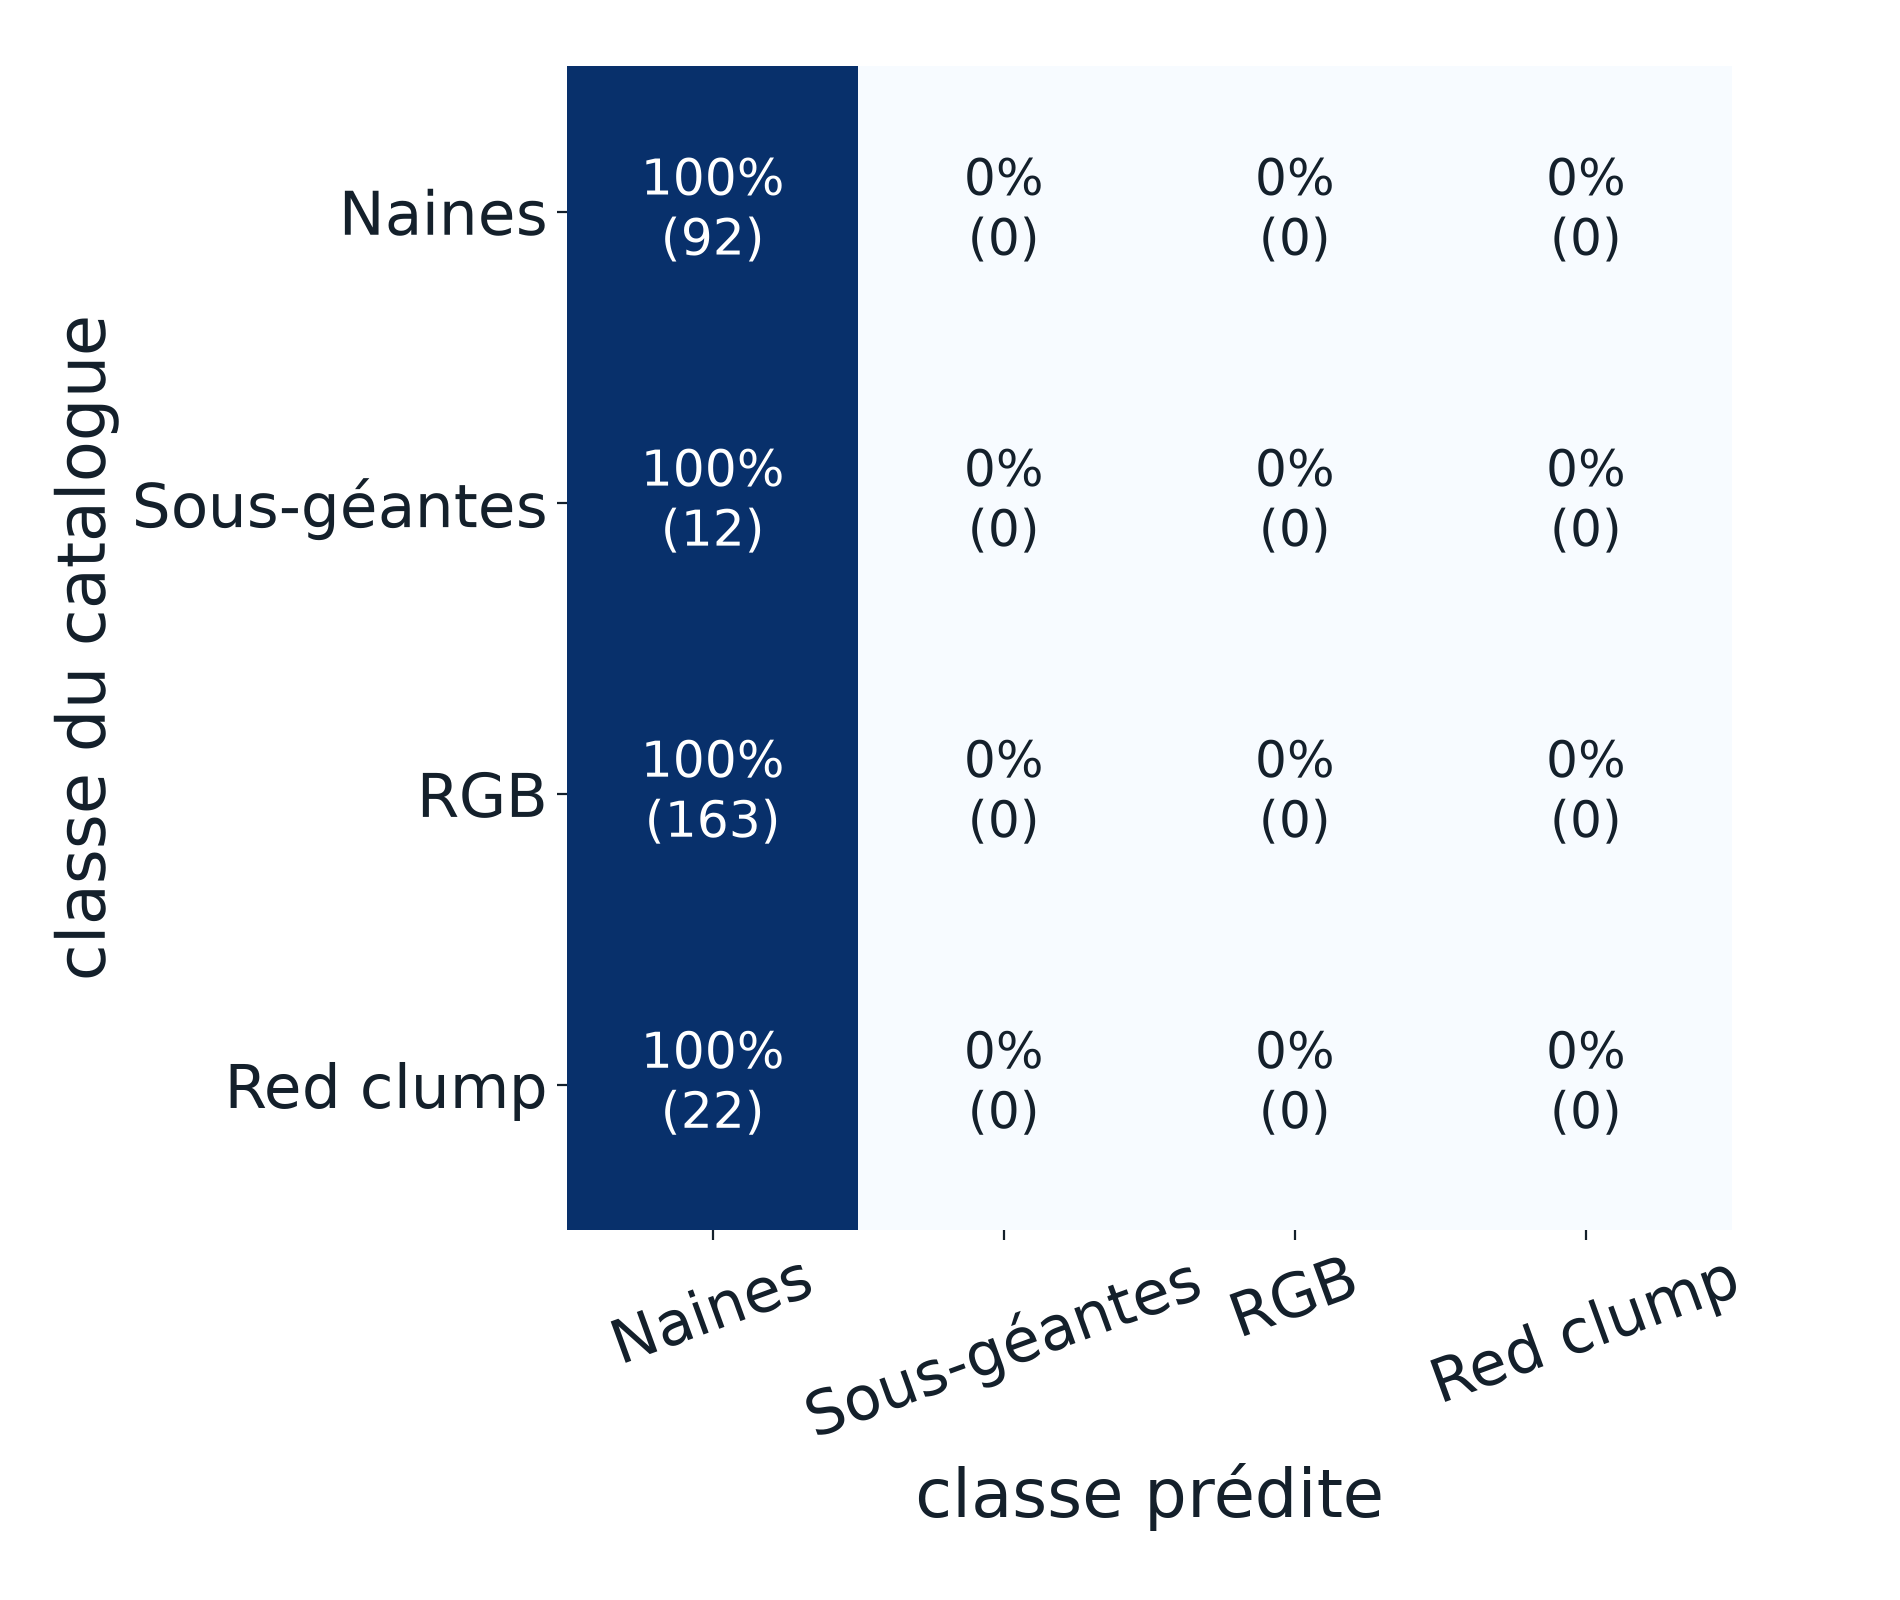
\includegraphics[width=0.52\linewidth]{confusion_cnn.png}
\caption{Matrice de confusion du CNN entraîné sur les bons spectres, sur \texttt{test\_good}.}
\label{fig:confusion}
\end{figure}

La matrice de confusion (figure~\ref{fig:confusion}) montre la même limite qu'en première version. Le CNN reconnaît 99\,\% des naines et 93\,\% des RGB, mais seulement 60\,\% du red clump : 40\,\% sont classées RGB. La différence entre ces deux classes tient au cœur de l'étoile et laisse peu de traces dans le spectre de surface.

\subsection{Impact de la qualité des données}

L'effet des mauvais spectres dépend de la tâche.

\paragraph{Classification.} Entraîner sur tous les spectres améliore le macro F1 du CNN de 0,834 à 0,860 sur \texttt{test\_good}, et de 0,806 à 0,838 sur \texttt{test\_all}. Le gain apparaît dans toutes les tranches de SNR (tableau~\ref{tab:snr}).

\paragraph{Régression.} Entraîner sur tous les spectres réduit l'erreur sur les spectres bruités, mais l'augmente sur les bons : \teff{} passe de 32,9 à 53,7\,K et \logg{} de 0,069 à 0,102\,dex sur \texttt{test\_good}. La forêt aléatoire, elle, profite des mauvais spectres (\teff{} de 30,0 à 28,1\,K).

\begin{table}[H]
\centering
\begin{tabular}{lrrrrrrr}
\toprule
SNR & $n$ & F1 bons & F1 tous & \logg{} bons & \logg{} tous & \teff{} bons & \teff{} tous \\
\midrule
5 à 30 & 396 & 0,42 & 0,52 & 0,65 & 0,53 & 650 & 590 \\
30 à 70 & 1\,093 & 0,71 & 0,76 & 0,18 & 0,17 & 191 & 141 \\
70 à 150 & 6\,297 & 0,78 & 0,81 & 0,089 & 0,111 & 71 & 71 \\
$> 150$ & 7\,182 & 0,84 & 0,87 & 0,078 & 0,106 & 77 & 60 \\
\bottomrule
\end{tabular}
\caption{CNN par tranche de SNR sur \texttt{test\_all}, selon le jeu d'entraînement. \logg{} en dex, \teff{} en K.}
\label{tab:snr}
\end{table}

\begin{figure}[H]
\centering
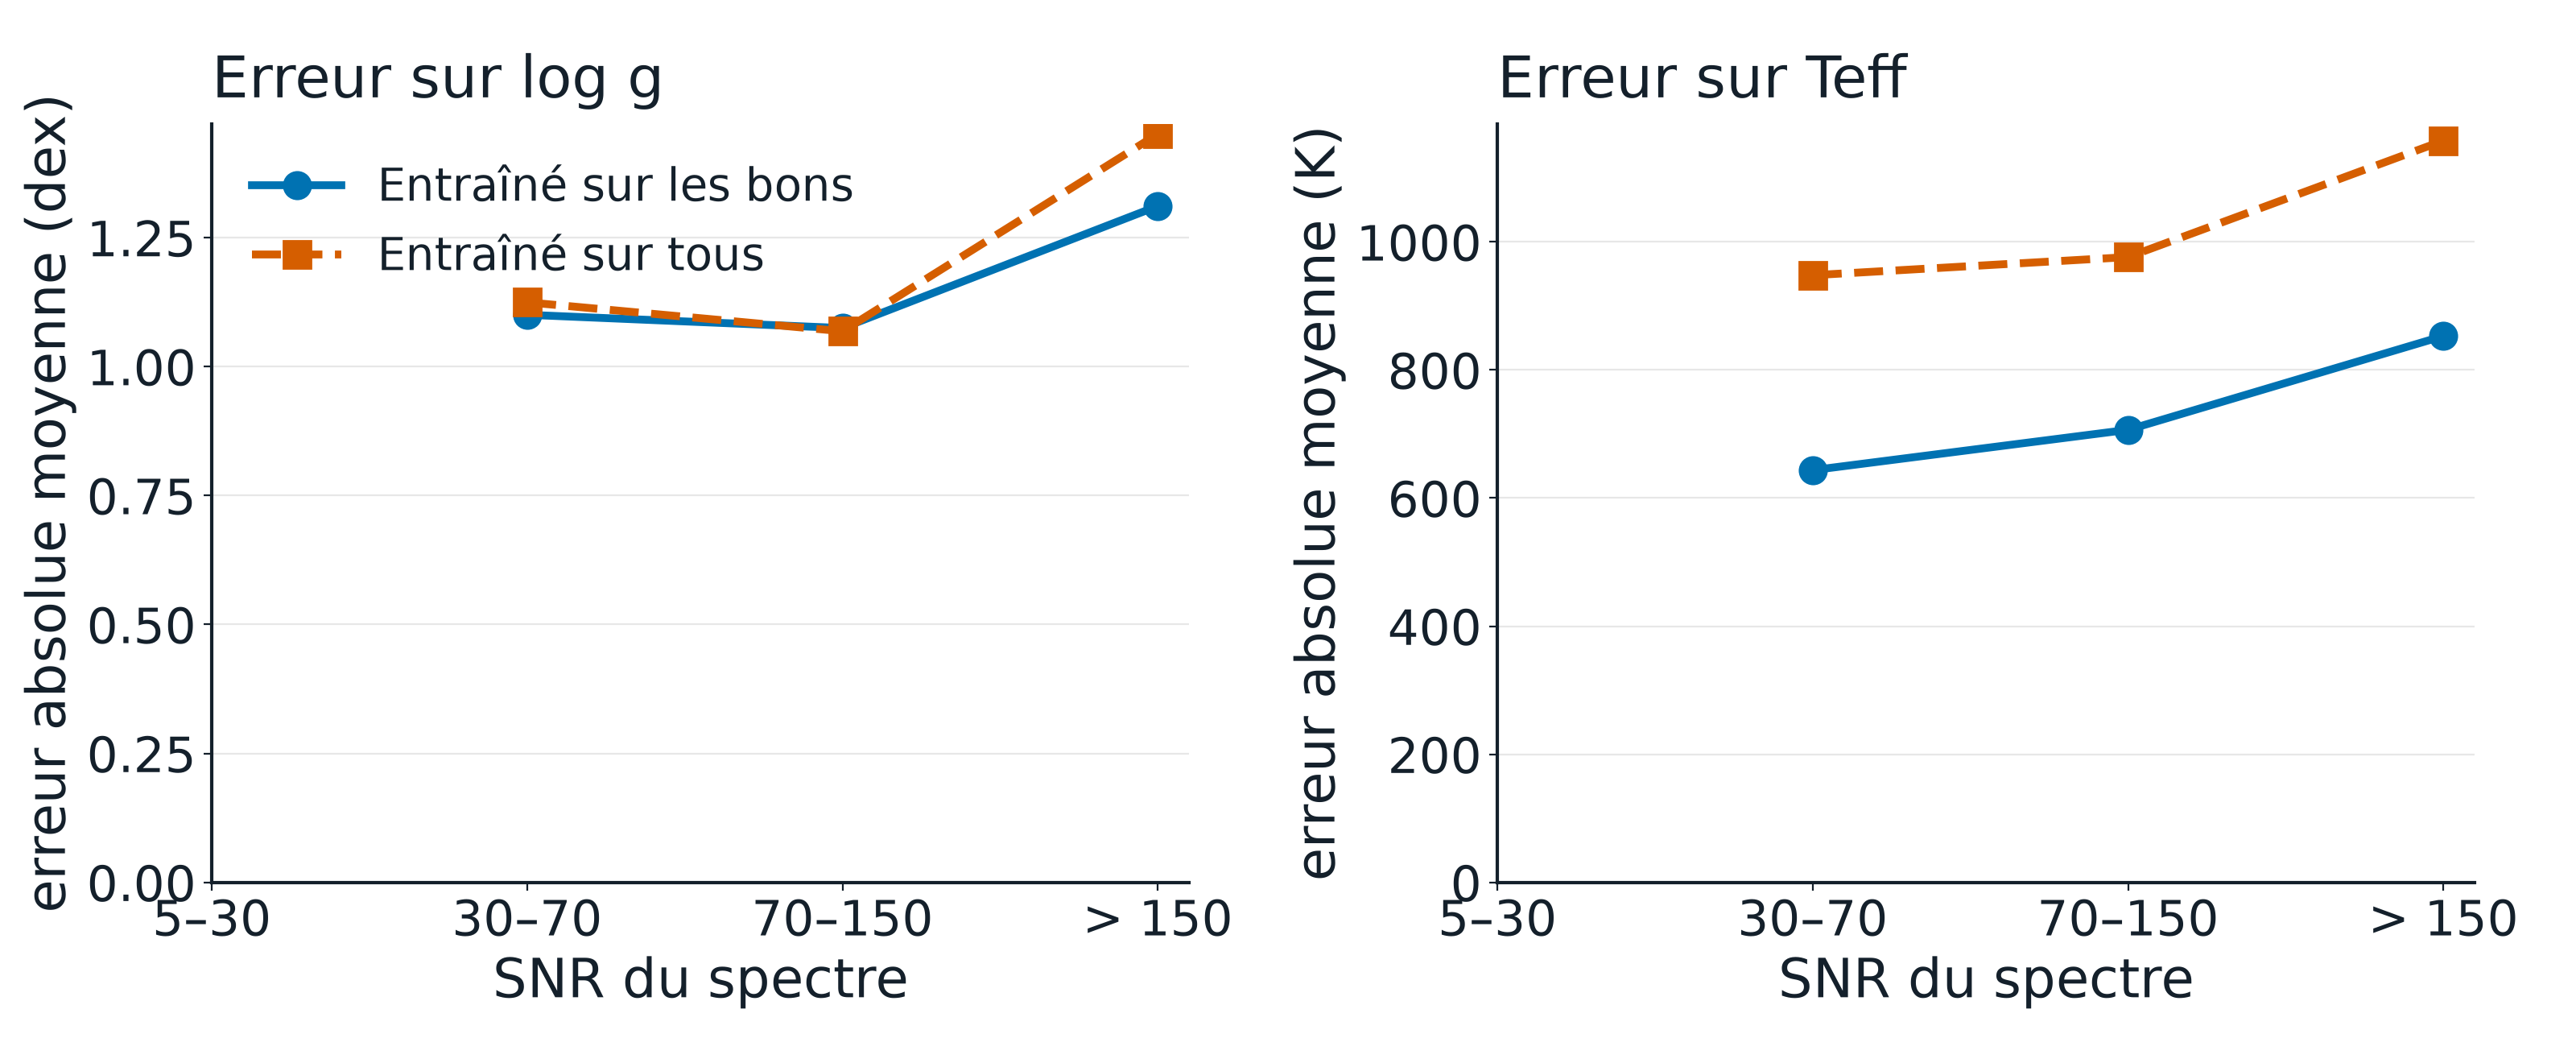
\includegraphics[width=\linewidth]{snr.png}
\caption{Erreur du CNN de régression par tranche de SNR sur \texttt{test\_all}.}
\label{fig:snr}
\end{figure}

\paragraph{Origine de l'erreur.} Le tableau~\ref{tab:source} sépare les erreurs selon l'origine de l'étiquette. Sur les 417 étoiles étiquetées par FPARAM, l'erreur sur \teff{} atteint 874\,K pour le modèle entraîné sur les bons spectres. Ces étiquettes sont peu fiables : ASPCAP a rejeté ces ajustements. Le modèle entraîné sur tous les spectres apprend une partie de ce bruit, ce qui dégrade ses prédictions sur les bons spectres.

\begin{table}[H]
\centering
\begin{tabular}{llrrrr}
\toprule
Étiquette & Qualité & $n$ & \teff{} bons (K) & \teff{} tous (K) & \logg{} bons / tous (dex) \\
\midrule
ASPCAP & bonne & 9\,997 & 32,9 & 53,7 & 0,069 / 0,102 \\
ASPCAP & mauvaise & 4\,554 & 170 & 117 & 0,143 / 0,142 \\
FPARAM & mauvaise & 417 & 874 & 470 & 0,565 / 0,452 \\
\bottomrule
\end{tabular}
\caption{Erreurs des CNN de régression sur \texttt{test\_all}, par origine d'étiquette et par qualité.}
\label{tab:source}
\end{table}

\subsection{Effet de la taille de l'échantillon}

\begin{table}[H]
\centering
\begin{tabular}{lrr}
\toprule
Mesure (\texttt{test\_good}, entraînement sur les bons) & 30\,781 étoiles & 99\,773 étoiles \\
\midrule
Macro F1, CNN & 0,818 & 0,834 \\
Macro F1, forêt & 0,696 & 0,751 \\
Erreur \teff{}, CNN (K) & 44,6 & 32,9 \\
Erreur \logg{}, CNN (dex) & 0,083 & 0,069 \\
Erreur \mh{}, CNN (dex) & 0,032 & 0,025 \\
Rappel du red clump, CNN & 56\,\% & 60\,\% \\
ARI, GMM sur PCA à $k = 3$ & 0,42 & 0,42 \\
ARI, GMM sur PCA à $k = 4$ & 0,09 & 0,44 \\
\bottomrule
\end{tabular}
\caption{Première version (allStarLite, 30\,781 étoiles) contre version complète.}
\label{tab:size}
\end{table}

Tripler l'échantillon améliore tous les modèles supervisés (tableau~\ref{tab:size}). La forêt gagne le plus (+0,055 de macro F1). Le clustering à $k = 3$ ne change pas : avec 20\,000 ou 66\,000 bons spectres, le GMM trouve les mêmes groupes. À $k = 4$, l'ARI passe de 0,09 à 0,44 : avec plus d'étoiles, le quatrième groupe du GMM se stabilise.

\subsection{Temps de calcul}

\begin{table}[H]
\centering
\begin{tabular}{lrr}
\toprule
Étape & Bons spectres (s) & Tous les spectres (s) \\
\midrule
Téléchargement des 99\,785 spectres & \multicolumn{2}{c}{5\,202 (une fois)} \\
PCA et t-SNE & \multicolumn{2}{c}{266 (une fois)} \\
Forêt aléatoire, classes & 80 & 23 \\
Forêt aléatoire, régression & 95 & 108 \\
CNN, classes (30 époques) & 249 & 323 \\
CNN, régression (30 époques) & 266 & 325 \\
Autoencodeur & 64 & 96 \\
Clustering sur PCA & 62 & 104 \\
Clustering sur le latent & 80 & 146 \\
\midrule
Total de l'expérience & \multicolumn{2}{c}{2\,374 (40 minutes)} \\
\bottomrule
\end{tabular}
\caption{Temps mesurés sur un portable avec une RTX 3060 (6\,Go), 16 threads et 15\,Go de mémoire.}
\end{table}

%=====================================================================
\section{Discussion}

\paragraph{Ce que le spectre contient.} La séparation naines / géantes émerge sans étiquette, et le CNN reconnaît 99\,\% des naines. La séparation red clump / RGB plafonne à 60\,\% de rappel, même avec trois fois plus de données.

\paragraph{Les mauvais spectres.} Un mauvais spectre apporte deux choses : un spectre bruité et une étiquette bruitée. La classification tolère le bruit d'étiquette : les classes suivent des seuils larges de \logg{}, et une erreur d'étiquette change rarement la classe. La régression le subit : le CNN reproduit les erreurs des étiquettes FPARAM et des ajustements rejetés. Pour la régression, la règle pratique devient : entraîner sur les spectres bruités, mais seulement avec des étiquettes fiables.

\paragraph{La taille de l'échantillon.} Les gains de 30\,000 à 100\,000 étoiles restent modestes pour le CNN (+0,016 de macro F1). Le plafond vient des étiquettes et de la physique (red clump / RGB), pas du volume.

%=====================================================================
\section{Limites et travaux futurs}

\begin{itemize}
  \item Les étiquettes viennent d'ASPCAP. Le CNN apprend à reproduire ASPCAP.
  \item Chaque modèle s'entraîne avec une seule graine.
  \item Les distances Gaia des étoiles du bulbe restent incertaines.
  \item La pureté OCCAM reste peu exigeante avec 2 à 4 groupes.
\end{itemize}

Travaux futurs, par ordre de priorité :
\begin{enumerate}
  \item Entraîner la régression sur tous les spectres, mais avec les étiquettes ASPCAP seulement, pour séparer l'effet du spectre bruité de celui de l'étiquette bruitée.
  \item Répéter chaque entraînement avec 5 graines.
  \item Valider la séparation red clump / RGB par astérosismologie.
  \item Rendre le clustering robuste aux valeurs extrêmes.
\end{enumerate}

%=====================================================================
\section{Conclusion}

Sur 99\,773 spectres APOGEE, le spectre seul sépare naines et géantes sans étiquette : un GMM sur PCA atteint un ARI de 0,44. Avec étiquettes, un CNN 1-D atteint un macro F1 de 0,86. Les mauvais spectres aident la classification et nuisent à la régression, parce que leurs étiquettes sont bruitées. Tripler l'échantillon améliore les modèles supervisés, mais ne lève pas la limite red clump / RGB.

\section*{Reproductibilité}
\addcontentsline{toc}{section}{Reproductibilité}

Le code se trouve dans le dépôt \url{https://github.com/imranakki/apogee-stars-full}. La première version reste dans \url{https://github.com/imranakki/apogee-stars}.

\begin{lstlisting}
export STARS_DATA=/chemin/vers/un/disque/avec/20Go
pip install -r requirements.txt
python scripts/01_get_catalogs.py
python scripts/02_select_stars.py
python scripts/03_download_spectra.py --workers 24
python scripts/04_explore.py
bash scripts/run_quality_experiment.sh
python scripts/10_label_source.py
python report/make_figures.py
\end{lstlisting}

\begin{thebibliography}{99}
\bibitem{dr17} Abdurro'uf et al. (2022). The Seventeenth Data Release of the Sloan Digital Sky Surveys. \textit{ApJS}, 259, 35.
\bibitem{majewski2017} Majewski, S. R. et al. (2017). The Apache Point Observatory Galactic Evolution Experiment (APOGEE). \textit{AJ}, 154, 94.
\bibitem{aspcap} García Pérez, A. E. et al. (2016). ASPCAP: The APOGEE Stellar Parameter and Chemical Abundances Pipeline. \textit{AJ}, 151, 144.
\bibitem{garciadias2018} Garcia-Dias, R., Allende Prieto, C., Sánchez Almeida, J. et Ordovás-Pascual, I. (2018). Machine learning in APOGEE: Unsupervised spectral classification with K-means. \textit{A\&A}, 612, A98.
\bibitem{bovy2014} Bovy, J. et al. (2014). The APOGEE Red-clump Catalog. \textit{ApJ}, 790, 127.
\bibitem{occam} Myers, N. et al. (2022). The Open Cluster Chemical Abundances and Mapping Survey. VI. Galactic Chemical Gradient Analysis from APOGEE DR17. \textit{AJ}, 164, 85.
\bibitem{weinberg2019} Weinberg, D. H. et al. (2019). Chemical Cartography with APOGEE: Multi-element Abundance Ratios. \textit{ApJ}, 874, 102.
\bibitem{tsne} van der Maaten, L. et Hinton, G. (2008). Visualizing Data using t-SNE. \textit{JMLR}, 9, 2579--2605.
\bibitem{hdbscan} Campello, R. J. G. B., Moulavi, D. et Sander, J. (2013). Density-Based Clustering Based on Hierarchical Density Estimates. \textit{PAKDD}, LNCS 7819, 160--172.
\bibitem{ari} Hubert, L. et Arabie, P. (1985). Comparing partitions. \textit{Journal of Classification}, 2, 193--218.
\end{thebibliography}

\end{document}
